\section{Runtime View}

\subsection*{Log in}
\begin{figure}[H]
	\centering
	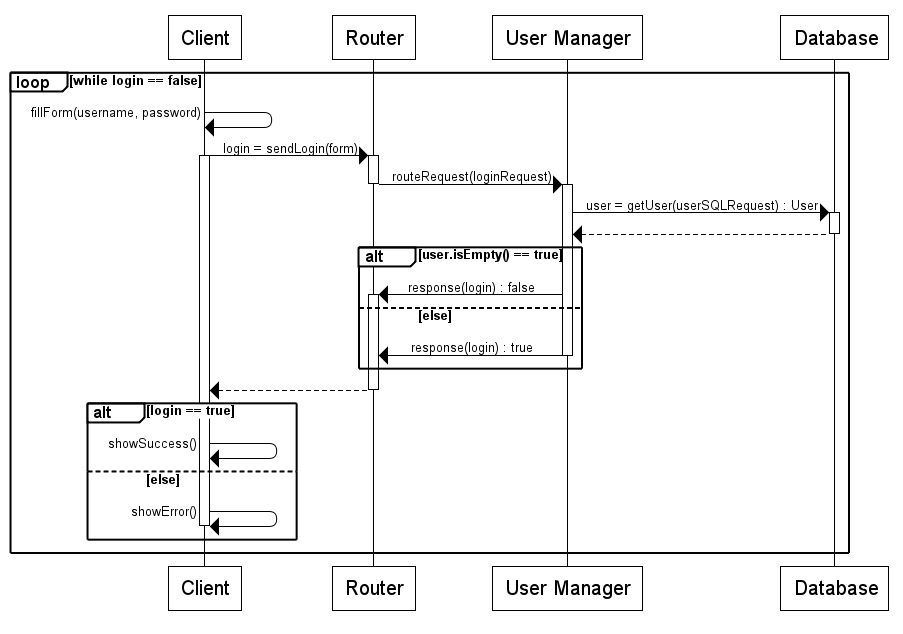
\includegraphics[width=1.4\textwidth, angle=90]{sequence-diagrams/login}
	\caption[Runtime View - Log in]{}
	\label{fig:login}
\end{figure}

\subsection*{Book a car}
\begin{figure}[H]
	\centering
	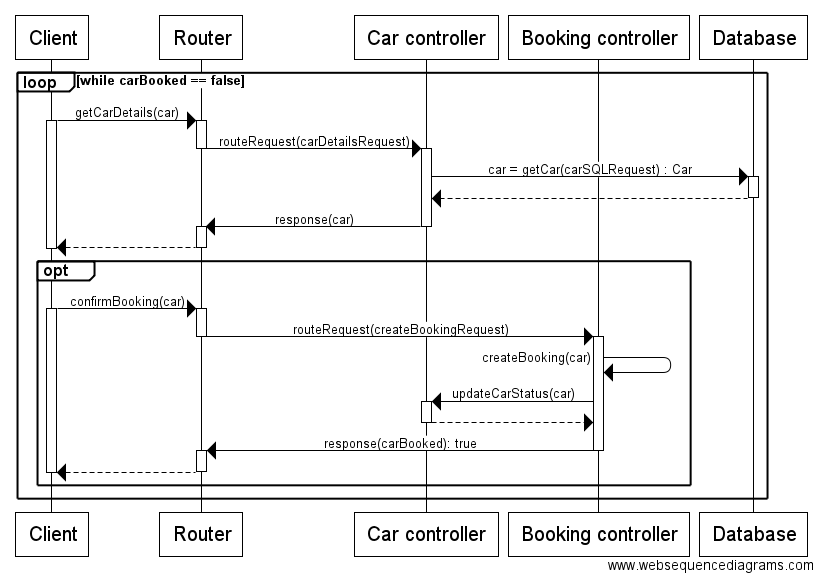
\includegraphics[width=1.4\textwidth, angle=90]{sequence-diagrams/booking}
	\caption[Runtime View - Book a car]{}
	\label{fig:booking}
\end{figure}

\subsection*{Cancel booking (elapsed time)}
\begin{figure}[H]
	\centering
	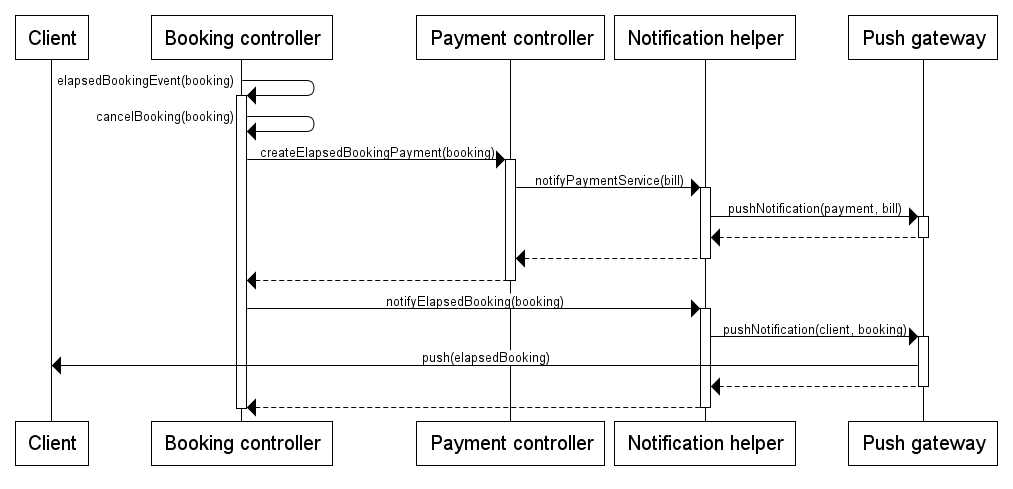
\includegraphics[width=1.4\textwidth, angle=90]{sequence-diagrams/cancel-booking-time}
	\caption[Runtime View - Cancel booking (elapsed time)]{}
	\label{fig:cancel-booking-time}
\end{figure}

\subsection*{Unlock car doors}
\begin{figure}[H]
	\centering
	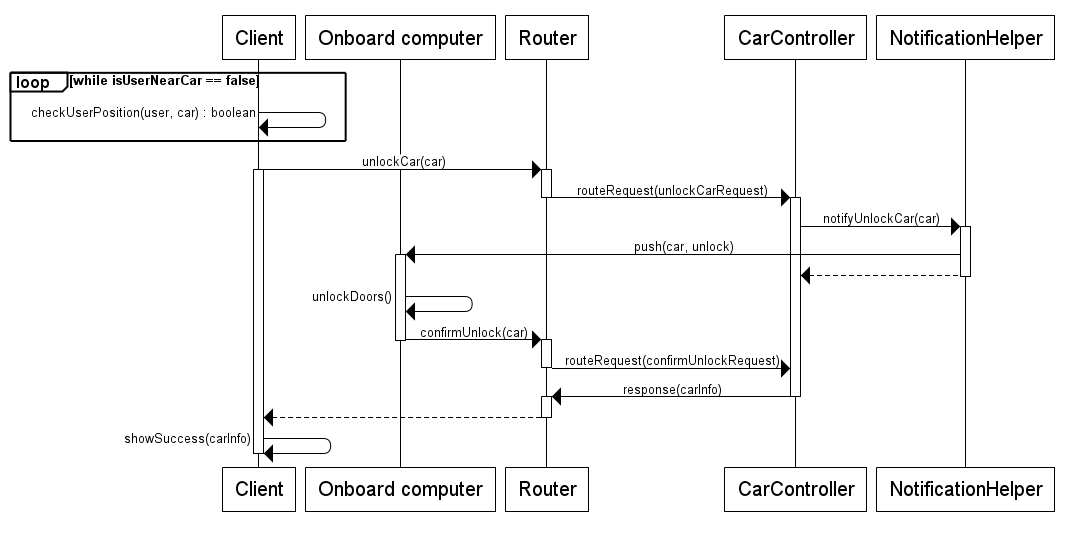
\includegraphics[width=1.4\textwidth, angle=90]{sequence-diagrams/open-car}
	\caption[Runtime View - Unlock car doors]{}
	\label{fig:open-car}
\end{figure}

\subsection*{Begin rental}
\begin{figure}[H]
	\centering
	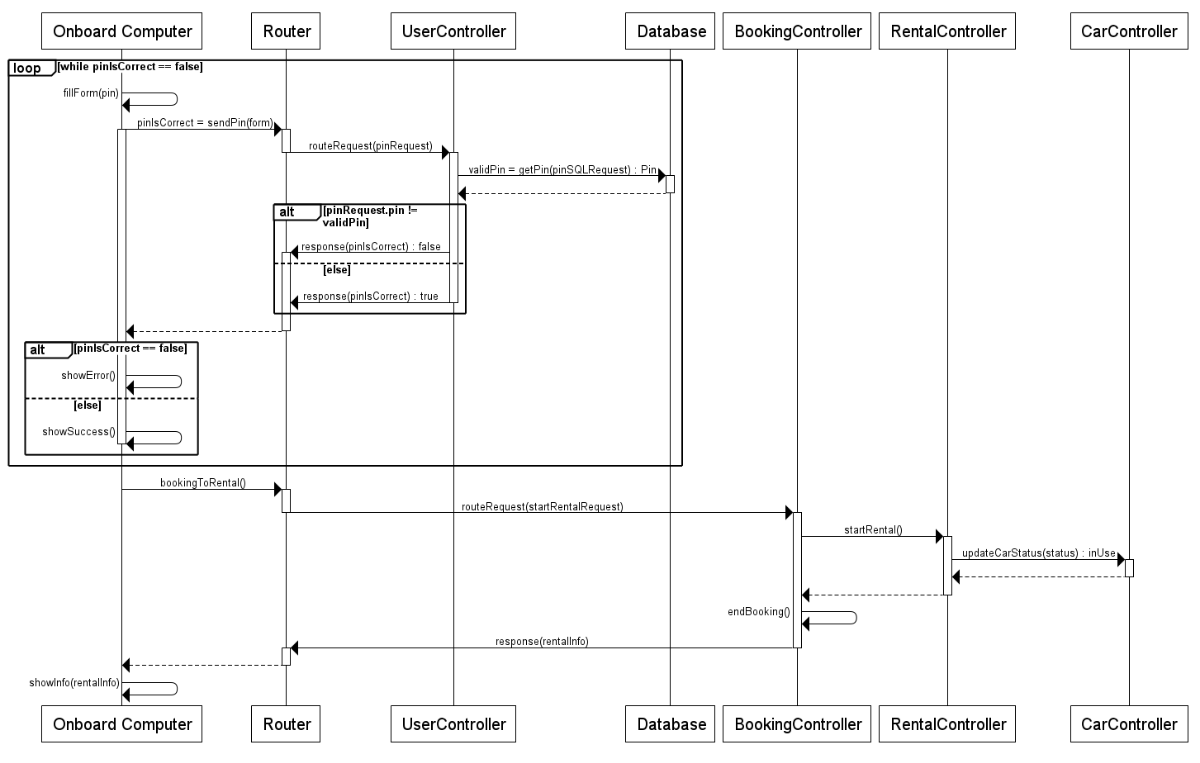
\includegraphics[width=1.4\textwidth, angle=90]{sequence-diagrams/begin-rental}
	\caption[Runtime View - Begin rental]{}
	\label{fig:begin-rental}
\end{figure}

\subsection*{End rental}
\begin{figure}[H]
	\centering
	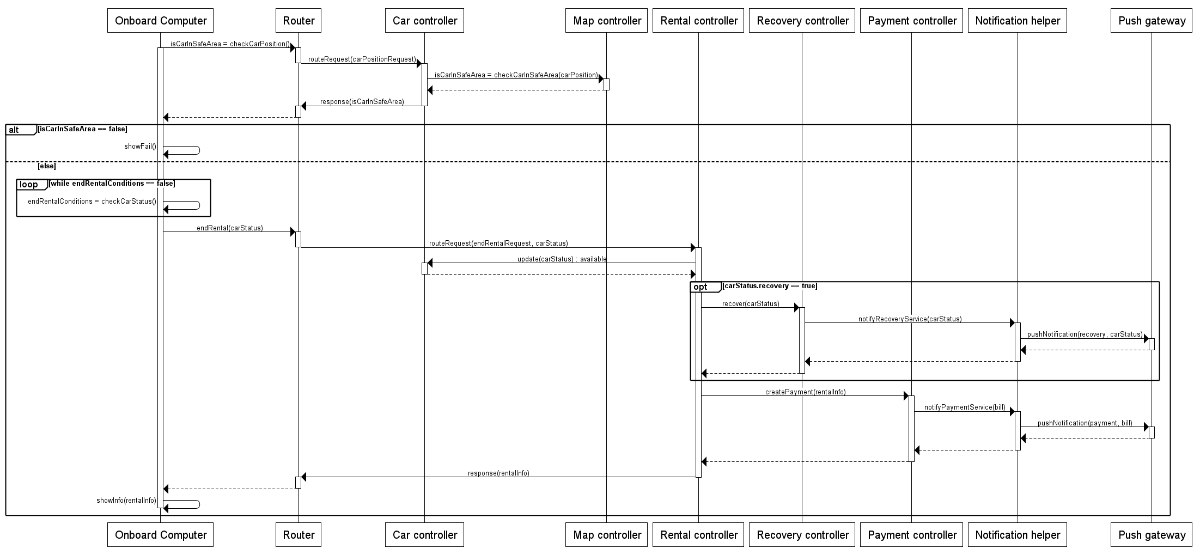
\includegraphics[width=1.4\textwidth, angle=90]{sequence-diagrams/end-rental}
	\caption[Runtime View - End rental]{}
	\label{fig:end-rental}
\end{figure}